\subsection{Quisquis}

Quisquis \cite{fauzi2019quisquis} is another approach to the construction of a decentralized private payment system. It's goal is to implement such a system without the disadvantages of the aforementioned systems. These drawbacks relate to the trusted setup of zk-SNARKs and the limited storage scalability of the ever-growing list of UTXO set. 

Quisquis working model is a hybrid one.In other words, it combines the account model, since each user has several accounts with its corresponding balance, with the UTXO logic, since transactions contain UTXO entries rather than accounts.This is made possible by the use of updatable public keys, a primitive that makes it possible to have a number of different public keys associated with the same private key. All of these keys are derived from the same original public key. In this way, a user can use the same private key to spend all of the UTXOs (denoted by the updated keys) that belong to his or her account. Each public key is used a maximum of twice, once during its generation on the output side and once during its use on the input side of a transaction.

Anonymity is achieved through the combination of anonymity sets with the use of the updatable public key primitive. More specifically, transactions can be thought of as "wealth redistribution" between inputs and outputs \autoref{fig:quisquis-redist-of-value}. Input accounts include the senders, the recipients as well as an anonymity set. Output accounts are new, updated but unlikable accounts for the senders, recipients, and decoys.

Confidentiality is achieved through a commitment scheme. Both the balances in the accounts and the transacted amounts are given in a commitment form. A user can change the corresponding commited value using the homomorphic property of the commitment scheme.

Finally, each transaction includes zero-knowledge proofs derived from $\Sigma$-protocols in order to ensure its validity.

\begin{figure}
    \centering
    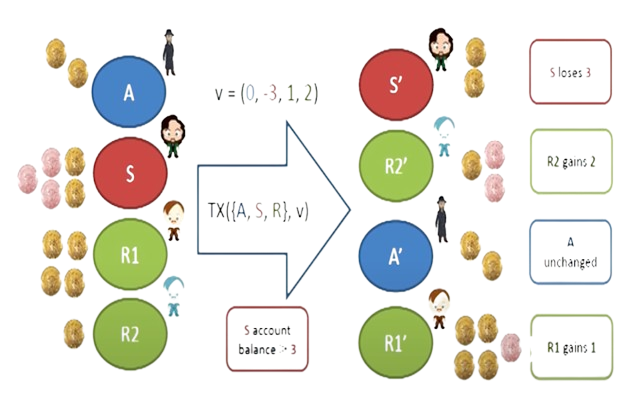
\includegraphics[width=0.8\textwidth]{images/quisquis/redist-of-value.png}
    \caption{Example of redistribution of value in Quisquis}
    \label{fig:quisquis-redist-of-value}
\end{figure}

\subsubsection{Updatable Public Keys} \label{UPK}

% We utilize the Updatable Public Key (UPK) primitive from~\cite{fauzi2019quisquis} to implement accounts. 
The concept of an UPK scheme is that public keys can be updated while remaining indistinguishable from freshly generated keys.
A UPK scheme is a tuple of algorithms $(\setup, \kgen, \upd, \verkp, \verupd)$. 
% The construction from~\cite{fauzi2019quisquis} operates over a prime-order group $(\group, g, p)$. 

\begin{itemize}
    \item $\setup$ generates the public parameters, which are implicitly given as input to all other algorithms, i.e. $\params \gets \setup(\secpar)$. For instance, \params\ could be a prime-order group $(\group, g, p)$.
    \item $\kgen$ generates a keypair $(\pk,\sk)$.
    Concretely, it is implemented as:
    Sample $r, \sk \sample \mathbb{F}_p$, calculate $\pk = (g^r, g^{r \dot \sk})$ and output $(\sk,\pk)$.
    \item $\upd$ takes as input a set of public keys $\{\pk\}_{i=1}^n$ and a secret key and generates a new set $\{\pk'\}_{i=1}^n$ where $\pk'_i = \pk_i ^ r = (g_i^r, g_i^{r \cdot \sk})$ for all $i$.
    \item $\verkp$ takes as input a keypair $(\sk, \pk)$ and checks if it is valid, i.e. if $\pk$ corresponds to $\sk$.
    It is constructed by parsing $\pk=(g',h')$ and outputting the result of the check $(g')^\sk \overset{?}{=} h'$.
    \item $\verupd$ takes as input a pair of public keys and some randomness $(\pk', \pk, r)$ and checks if $\pk'$ is a valid update of $\pk$ using $r$. This is done by checking if $\upd(\pk;r) \overset{?}{=} \pk'$.
\end{itemize}

An UPK scheme must satisfy the following properties:
\begin{itemize}
    \item \textbf{Correctness}: All honestly generated keys verify correctly, the update process can be verified and the updated keys also verify successfully.
    \begin{definition}\label{def:UPKCorrectness} 
        A UPK satisfies perfect correctness if the following three properties hold for all $(\pk, \sk) \in [\kgen]$:
        \begin{itemize}
            \item $\verkp(\pk,\sk) = 1;$
            \item $\verupd(\upd(\pk;r), \pk, r) = 1 \ \forall r  \in \rset;$
            \item $\verkp(\pk^\prime, \sk) = 1 \ \forall \pk^\prime \in [\upd(\pk)].$
        \end{itemize}
    \end{definition}
    \item \textbf{Indistinguishability}, meaning that an adversary cannot distinguish between a freshly generated public key and an updated version of public key it already knows.
    \begin{definition}\label{def:UPKindistinguishability} 
        The \emph{advantage} of the adversary in winning the indistinguishability game \ref{alg:UPKindistinguishability-game} is defined as:
        $
            \advantage{ind}{\adv} = \mid \Pr[\exper^{ind}_{\adv}((\secpar))=1] - \dfrac{1}{2} \mid
        $
    
        A DPS satisfies \emph{indistinguishability} if for every PPT adversary $\adv$, $\advantage{ind}{\adv}$ is negligible in  $\secpar$.
    \end{definition}
    \begin{game}[htbp]
        \DontPrintSemicolon
        \SetAlgoLined
        \caption{Indistinguishability game $\exper^{ind}_{\adv}(\secpar)$}
        \label{alg:UPKindistinguishability-game}
        \SetKwInOut{Input}{Input}
        \SetKwInOut{Output}{Output}
        \Input{$\secpar$}
        \Output{$\{0,1\}$}
        \BlankLine
        $b\gets \{0, 1\}$ \;
        $(\pk^*, \sk^*) \gets \kgen()$\;
        $r \sample \randspace$\;
        $\pk_0 \gets \upd(\pk^*;r)$\;
        $(\pk_1, \sk_1) \gets \kgen()$\;
        $b^\prime \gets \adv(\pk^*, \pk_b)$\;
        \Return{$(b = b^\prime)$}
    \end{game}
    Note that in indistinguishability game \ref{alg:UPKindistinguishability-game} the challenger can update many times the $\pk^*$ before creating $\pk_0$ due to the fact that even with more updates the $pk_0$ can be described as an update of $\pk^*$ with a different randomness.
    \item \textbf{Unforgeability}, meaning that for every honestly generated keypair an adversary cannot learn the secret key of an updated public key without knowing the secret key of the original public key. This is formalized by saying that the adversary cannot generate a public key for which he knows both the secret key and the randomness required to explain that public key as an update of an honestly generated public key.
    \begin{definition}\label{def:UPKunforgeability} 
        The \emph{advantage} of the adversary in winning the unforgeability game \ref{alg:UPKunforgeability-game} is defined as:
        $
            \advantage{unf}{\adv} = \mid \Pr[\exper^{unf}_{\adv}((\secpar))=1] - \dfrac{1}{2} \mid
        $
    
        A DPS satisfies \emph{unforgeability} if for every PPT adversary $\adv$, $\advantage{unf}{\adv}$ is negligible in  $\secpar$.
    \end{definition}
    \begin{game}[htbp]
        \DontPrintSemicolon
        \SetAlgoLined
        \caption{Unforgeability game $\exper^{unf}_{\adv}(\secpar)$}
        \label{alg:UPKunforgeability-game}
        \SetKwInOut{Input}{Input}
        \SetKwInOut{Output}{Output}
        \Input{$\secpar$}
        \Output{$\{0,1\}$}
        \BlankLine
        $(\pk, \sk) \gets \kgen()$\;
        $(\sk^\prime, \pk^\prime, r) \gets \adv(\pk)$\;
        \Return{$\verkp(\pk^\prime, \sk^\prime) \land \verupd(\pk^\prime, \pk, r)$}
    \end{game}
\end{itemize}

If the $\ddh$ assumption holds in $(\group, g, p)$ then this construction satisfies correctness, indistinguishability and unforgeability.

\begin{proof}
Correctness is straightforward to verify. Indistinguishability derives from the DDH assumption. An adversary $\adv$ that can win the indistinguishability game \ref{alg:UPKindistinguishability-game} can be used to create $\badv$ who can distinguish a DDH tuple. That can be proven using the following reduction \ref{alg:UPK-ind-adv}. 

\begin{algorithm}[htbp]
    \caption{Adversary who wins DDH: $\badv(chl)$}
    \label{alg:UPK-ind-adv}
    \DontPrintSemicolon
    \SetAlgoLined
    \SetKwInOut{Input}{Input}
    \SetKwInOut{Output}{Output}
    \Input{$chl  = (g,g^x,g^y, g^z)$}
    \Output{$\{0,1\}$}
    \BlankLine
    $r \sample \randspace$\;
    $\pk^* = (g^r, g^{xr})$\;
    $\pk^\prime = (g^{yr}, g^{zr})$\;
    $b \gets \adv(\pk^*, \pk^\prime)$\;
    \Return{$b$}

\end{algorithm}
If $chl$ is a DDH tuple then $\pk^\prime$ is distributed identically to $\pk_0$. Otherwise $\pk^\prime$ is distributed identically to $pk_1$. Therefore, the reduction has the same non-negligible advantage in the DDH as the $\adv$ has in the indistinguishability game \ref{alg:UPKindistinguishability-game}.

Unforgeability derives from the DL assumption. An adversary $\adv$ that can win the unforgeability game \ref{alg:UPKunforgeability-game} can be used to create $\badv$ who can win the DL game. That can be proven using the following reduction \ref{alg:UPK-unf-adv}. 

\begin{algorithm}[htbp]
    \caption{Adversary who wins DL: $\badv(chl)$}
    \label{alg:UPK-unf-adv}
    \DontPrintSemicolon
    \SetAlgoLined
    \SetKwInOut{Input}{Input}
    \SetKwInOut{Output}{Output}
    \Input{$chl  = (g, h = g^s)$}
    \Output{$s$}
    \BlankLine
    $t \sample \randspace$\;
    $(g_0, h_0) = (g^t, h^t)$\;
    $\pk = (g_0, h_0)$\;
    $(\sk^\prime, \pk^\prime = (g_1, h_1), r) \gets \adv(\pk)$\;
    \Return{$\sk^\prime$}

\end{algorithm}
The winning condition of the unforgeability definition \ref{def:UPKunforgeability} requires that $(h_1 = g_1 ^ {\sk^\prime})$ and $(g_1, h_1) = (g_0^r, h_0^r) = (g^{rt}, h^{rt})$ thus implying that $g^{\sk\prime r t} = h^{rt}$ or equivalent that $h = g^{\sk^\prime}$, meaning $\sk^\prime = s$ or that it is a valid solution to the DL oracle.

\end{proof}

